% \documentclass[algorithmlist,figurelist,tablelist,nomlist]{template/seumasterthesis} %学硕使用这一行
\documentclass[algorithmlist,figurelist,tablelist,nomlist,engineer]{template/seumasterthesis}
\usepackage{multirow} % 处理跨行表格数据
\usepackage{float}
\usepackage{lipsum}
\usepackage{pifont}  % 引入 pifont 宏包
\usepackage{enumitem}
\renewcommand{\thefootnote}{\ding{\numexpr171+\value{footnote}}}
\setCJKmainfont{simsun.ttc}[AutoFakeBold]
\begin{document}

%% ----------------------------------------------------------------------------
%%                                 Meta Data
%% ----------------------------------------------------------------------------
\categorynumber{TN92} %《中国图书资料分类法》分类法
\UDC{621.3}              %《国际十进分类法UDC》的类号
\secretlevel{公开}        % 学位论文密级分为"公开"、"内部"、"秘密"和"机密"四种
\studentid{220000}      % 学号要完整,前面的零不能省略

%% ----------------------------------------------------------------------------
%%                           Thesis Title and Spine
%% ----------------------------------------------------------------------------
\title
    {东南大学 \LaTeX 论文模板使用手册}        % 论文中文标题
    {如何优雅地撰写硕士研究生毕业论文}         % 论文中文副标题,没有可以空着
    {Southeast University \LaTeX ~Thesis Template User Manual}  % 论文英文标题
    {How to Write a Master Thesis in an Elegant Way}            % 论文英文副标题,没有可以空着

\spine
	% 书脊标题与副标题
    {东南大学 \rotatebox{270}{\raisebox{2.5pt}{LaTeX}} 论文模板使用手册} 
    {}                                                               

%% ----------------------------------------------------------------------------
%%                             Author and Advidor
%% ----------------------------------------------------------------------------
\author
    {王东南}                        % 作者中文姓名
    {XX Xxxx}                  % 作者英文姓名,首字母大写,姓名分开,双字用「-」连接

\advisor
    {王东南 教授}                % 导师中文姓名
    {YY Yyyy}        % 导师英文姓名
    {Prof.}                     % 导师职称
    
\coadvisor                 % 联合培养导师姓名,没有可以不写
    {王东南 高工}                  % 导师中文姓名
    {ZZ Zzzz}             % 导师英文姓名
    {Eng.}                 % 导师职称 (English), 如教授(Prof.)、副教授(A.P.)
%% ----------------------------------------------------------------------------
%%                              Thesis Defence
%% ----------------------------------------------------------------------------
\engthesistype{应用研究}            % 工程硕士论文类型
\degreetype                        % 学位类型
    {电子信息硕士}
    {Master of Electronic Information}
\major{ \begin{minipage}{\linewidth}\centering 通信工程(含宽带\\网络、移动通信等)\end{minipage}}                 % 一级学科名
\submajor{通信与信息系统}             % 二级学科名
\defenddate{2025年5月18日}          % 答辩日期 \today
\authorizedate{}                  % 授予学位日期,这个档案袋不需要填
\committeechair{}               % 答辩委员会主席姓名
\reviewer{}{}                % 两位论文评阅人姓名
\department                        % 学院名称
    {信息科学与工程学院}
    {School of Information Science and Engineering}
% \seuthesisthanks                % 资助信息,没有可以不写
%     {本文的部分工作受国家自然基金 No. zxgg666 的支持与帮助,在此表示感谢。}

%garbagecoder: \let 是 TeX 的赋值命令,它会让 \cleardoublepage 变成 \clearpage,原模板限制奇偶页适用于双面打印,此命令用于去掉多余的空白页
% \let\cleardoublepage\clearpage 

%% ----------------------------------------------------------------------------
%%                                  Cover
%% ----------------------------------------------------------------------------
% ⚠️ 可以在编写论文的时候注释掉封面,加快编译速度
\makebigcover  % 生成A3大封面
\makecover     % 生成小封面
	 
%% ----------------------------------------------------------------------------
%%                          Abstract and Contents
%% ----------------------------------------------------------------------------
%% ----------------------------------------------------------------------------
%%                              Chinese Abstract
%% ----------------------------------------------------------------------------
\begin{abstract}{\TeX, \LaTeX, 学位论文}
本文提出了一个新的东南大学 \LaTeX 硕士研究生毕业论文模板,并说明了如何更优雅地写出一篇漂亮而无用的文章。
\end{abstract}

%% ----------------------------------------------------------------------------
%%                              English Abstract
%% ----------------------------------------------------------------------------
\begin{englishabstract}{\TeX, \LaTeX, Thesis}
This article proposes a new Southeast University master degree thesis \LaTeX ~template and explains how to elegantly write an article which is beautiful but full of shit.
\end{englishabstract}

\cleardoublepage
\addcontentsline{toc}{chapter}{目  录}
\tableofcontents          % 生成目录
\listofothers             % 生成图、表等目录,没有可以不写
 
%% ----------------------------------------------------------------------------
%%                                Main Body
%% ----------------------------------------------------------------------------
\mainmatter                    % 开始正文
\chapter{模板的安装与使用}
\label{chp:installation}

本章将介绍如何配置 \LaTeX 开发环境并使用本模板编译PDF格式的论文。
\nomenclature{PDF}{Portable Document Format\nomchinese{便携式文档格式}}
\nomenclature{6G}{6th Generation Mobile Communication\nomchinese{第六代移动通信}}

\section{注意事项}

\textbf{加粗的字体示例。在Windows下,加粗宋体字体异常,本模板使用AutoFakeBold来表示加粗宋体。}

参考文献示例\cite{JSJX202411005}参考文献\citet{JSJX202411005}参考文献\citen{JSJX202411005}参考文献。

参考文献\cite{tseng2021codedbulk}参考文献\citet{tseng2021codedbulk}参考文献\citen{tseng2021codedbulk}参考文献。
该模板下,中英文参考文献只保留前三位作者,第四位及以后的作者使用等或et al替代,参考附件3-GBT 7714-2015参考文献著录规则.pdf,英文作者姓名字母全部大写,会议[C]的后面使用.而不是//。

本模板将图、表列表中的内容修改为图1-1、表1-1的形式,原模板中的列表只有1-1,没有“图”、“表”字样。

本模板将原模板适用于双面打印的形式修改为单面,去掉了一些空白页。

\section{环境准备}
\label{sec:tex_environment}

使用本模板之前首先需要在你的设备上配置好 \LaTeX 开发环境。目前主流的计算机操作系统都对 \LaTeX 有较好的支持,接下来我们将以几个常见操作系统为例介绍环境的配置方法。

\subsection{Microsoft Windows\texttrademark}

\LaTeX 在Microsoft Windows操作系统上的发行版称为 Tex Live,该发行版提供了较为全面的现代 \LaTeX 编译引擎支持,包括了对 XeLaTeX 和 LuaTeX 的良好支持。需要强调的是,一些网络上的教程可能会指导初学者下载 CTeX 安装套件,请不要这样做。CTeX 是刀耕火种时代 \LaTeX 社群针对中文使用者发明的妥协产物,在早期有其使用价值,但现如今在使用时往往会面临宏包缺失和兼容性问题\cite{muzi2020ctex}。为了避免你在issue中反复抱怨编译错误,或者发邮件询问一个本不该出现的问题,请珍爱生命,使用 Tex Live。

截止到本文撰写的时间点,Tex Live的最新版本为Tex Live 2019,你可以在\href{http://tug.org/texlive/}{这个网站}找到下载链接。请尽量选择完全下载并本地安装而非使用下载器在线安装,因为大部分中国IP的连接速度让人绝望。下载时你可以就近选择节点,如果你使用的是校园网的话可以达到一个相当可观的下载速度。

安装过程较为简单,按照步骤设定安装位置即可。需要注意的是,请你在安装完成后设定好环境变量。尽管不设定环境变量在多数情况下也可以工作,但是你将无法使用我们提供的编译脚本。设定环境变量的方法与步骤不在本文的教程范围之内,请自行百度。

\subsection{Apple MacOS\texttrademark}

\LaTeX 在Apple MacOS操作系统上的发行版称为MacTeX。在 MacOS 上安装 MacTeX 之前,请确保你已经正确安装了\href{https://brew.sh/}{homebrew}。当然,你也可以直接从\href{http://www.tug.org/mactex/index.html}{官网}下载 MacTeX套件,但本文建议你使用 homebrew 安装纯净的 MacTeX 发行版。MacTeX 分为基本版和完全版,区别主要在于完全版中默认包含了更多的宏包。安装基本版 MacTeX 已经可以应付你绝大多数 \LaTeX 需求,在终端中输入:

\begin{tcolorbox}
\begin{lstlisting}
brew cask install basictex
\end{lstlisting}
\end{tcolorbox}

\noindent 你就可以获得了基本版的 MacTeX。如果你一定要安装完全版,请在终端中输入:

\begin{tcolorbox}
\begin{lstlisting}
brew cask install mactex
\end{lstlisting}
\end{tcolorbox}

\subsection{Ubuntu Linux}

在 Ubuntu 中配置 \LaTeX 开发环境最为简单。事实上如果你是一个 GNU/Linux 使用者,你应该已经具有了相当的工程能力能够自行配置 \LaTeX 编译环境。但为了本文结构上的完整,我们决定还是多此一笔。在终端中输入:

\begin{tcolorbox}
\begin{lstlisting}
sudo apt install texlive-full
\end{lstlisting}
\end{tcolorbox}

\noindent 你就可以在 Ubuntu 设备上部署 Tex Live 发行版。其他 Linux 发行版上的安装方法与 Ubuntu Linux 类似,只是各自使用的包管理器可能有所不同,请参阅各发行版的包管理中心网站,本文不再赘述。

\section{模板的下载与安装}
\label{sec:template_download}

其实在你看到本手册的同时,我们相信你已经成功地将本模版下载到了你的设备上。因此本来并没有必要在此赘述介绍工程的下载方法。但为了防止你下载的并非最新版本的模板工程,或者本模板被其他网站转载而你恰好从别的网站上下载了本模板,我们觉得还是有必要介绍一下我们指定的下载地址。本模板工程的所有代码都已经在GitHub上开源,你可以从\href{https://github.com/herculas/SEU-master-thesis}{这个地址}找到本模板的最新版本。

将本模板工程文件解压缩到你喜欢的目录下,你就得到了完整的模板工程。为了避免不必要的编译问题,我们建议你将工程保存在全英文的目录下。本模板已在 Windows 10,MacOS 10.15 Catalina,Ubuntu 18.04 Bionic Beaver以及Manjaro 19.0.2 上编译通过,但需要注意的是一些 Linux 发行版中没有安装本模板编译所需的字体文件,如宋体、黑体、楷体和 Times New Roman 等。因此如果你在 Linux 下遭遇了编译问题,请首先检查你的字体是否都已经安装完好。

\section{论文的编译}
\label{sec:compilation}

如果你使用的是如 Tex Studio,Texpad 或 WinEdt 等 \LaTeX 集成环境,你可以从这些软件中直接启动编译。但是作为一个较为庞大的、涉及多文件的 \LaTeX 工程,你可能需要多次编译才能获得完整的论文。一个完整的编译过程包含下面几个步骤:

\begin{tcolorbox}
\begin{lstlisting}
xelatex main
bibtex main
makeindex main.nlo -s nomencl.ist -o main.nls
xelatex main
xelatex main
\end{lstlisting}
\end{tcolorbox}

\noindent 想要编译一篇学位论文,首先需要对文章结构和原始文本进行一次预编译;随后索引出论文中出现的所有参考文献,并建立参考文献条目与论文引用位置的连接;接下来,根据预编译所产生的文章结构,需要生成文章的图表和术语索引文件;最后通过两次编译将参考文献和图表索引编入正文中,得到完整的PDF版本论文。可以看到这个过程极其复杂,因此我们为你准备了两个脚本文件,来将你从复杂的编译流程中解脱出来。对于 Windows 用户,你可以双击工程根目录下的 make.bat 文件启动编译流程。而 MacOS 和 Linux 用户则可以在命令行中执行根目录下的 make.sh 脚本来启动编译流程。

对于使用类 Unix 操作系统的用户,我们也在 3.4.3 版本之后加入了对 GNU Make 的支持,你现在可以使用 make 命令进行论文的自动化增量编译。GNU Make 工具和 make 命令的相关知识,可以参考\href{https://www.gnu.org/software/make/manual/make.html}{这里}。
      % 第一章:
\chapter{论文的初始化}
\label{chp:initialization}

在开始撰写学位论文之前,我们建议你首先对你论文的基本信息进行初始化。这部分的工作在main.tex文件中完成。接下来我们将详细介绍各部分的填写方法。注意,下列所有源代码中尖括号{\codefont <...>}里的内容代表你需要填写的文本。

\section{元数据}

元数据部分控制你论文A3封面和中文彩色封面左上角的论文元信息的显示,除固定的学校代码外分为4个部分。下面我们将逐一解释每个部分的填写规则。

\subsection{分类号}

分类号指代中国图书馆分类法 (CLC, Chinese Library Classification)对图书资料的分类编码,请根据你学术论文的内容与分类酌情填写。

\begin{tcolorbox}
\begin{lstlisting}[language=TeX]
\categorynumber{<CLC Code>}
\end{lstlisting}
\end{tcolorbox}

\noindent 举例来说,\textbf{网络安全}的中图法分类号为TN915.08,而\textbf{建筑水利工程}的分类号为F407.9。如对自己研究内容的具体分类不甚确定,可以参阅\href{https://www.clcindex.com/}{相关网站}。

\subsection{UDC}

UDC(Universal Decimal Classification)指通用十进制分类法,是国际上规模最大影响最广泛的文献资料分类法。在此部分你需要填写学术论文所属的十进制分类编码。

\begin{tcolorbox}
\begin{lstlisting}[language=TeX]
\UDC{<UDC Code>}
\end{lstlisting}
\end{tcolorbox}

\noindent 举例来说,\textbf{人工智能}的UDC分类号为004.8,而\textbf{凝聚态固态物理学}的分类号为538.9。如对自己研究内容的具体分类不甚确定,可以参阅\href{http://www.udcsummary.info/php/index.php?lang=chi}{相关网站}。

\subsection{保密级别}

在此部分你需要指定你的学术论文所属的保密级别。

\begin{tcolorbox}
\begin{lstlisting}[language=TeX]
\secretlevel{<Secret Level>}
\end{lstlisting}
\end{tcolorbox}

\noindent 一般的,学位论文的保密级别分为公开、内部、秘密和机密四级。具体区别在于:

\begin{itemize}
  \item \textbf{公开}:未涉及国家保密范围以及未准备申请专利权或技术转让的一般学术研究;
  \item \textbf{内部}:未涉及国家保密范围但准备申请专利权或技术转让的在一段时间内不适宜公开的学术研究;
  \item \textbf{秘密与机密}:涉及国家保密特定密级的科研项目或课题及其衍生的学术研究。
\end{itemize}

\noindent 请根据你的论文的具体情况酌情填写。

\subsection{学号}

在此部分你需要填写你的研究生学号。

\begin{tcolorbox}
\begin{lstlisting}[language=TeX]
\studentid{<Student ID>}
\end{lstlisting}
\end{tcolorbox}

\noindent 东南大学的研究生学号一般为6位数字,请注意不要与9位的一卡通号混淆。也请学号为8位数字的本科生同学关闭本文档,出门左转GitHub寻找适合本科生的论文模板。

\section{论文标题与书脊}

\subsection{中英文标题}

论文标题部分控制你论文的A3封面、中文彩色封面、中文内页封面和英文封面上的标题显示。

\begin{tcolorbox}
\begin{lstlisting}[language=TeX]
\title
    {弯扭耦合下土木工程复合材料梁的变分渐近模型}
    {}
    {Variational Asymptotic Model of Composite Beams Used in Civil Engineering under Bending and Torsion Coupling}
    {}
\end{lstlisting}
\end{tcolorbox}

\noindent 对论文标题的指定分为4个部分,自上而下分别是中文主标题,中文副标题,英文主标题和英文副标题。对于大多数没有副标题的学位论文,中英文副标题部分可以留空,但请务必不要删去相应的括号。有些论文的中英文标题可能过长,这时你也可以使用副标题位置来实现更加灵活自主的换行。比如上面的示例可以改写成:

\begin{tcolorbox}
\begin{lstlisting}[language=TeX]
\title
    {弯扭耦合下土木工程复合材料梁}
    {的变分渐近模型}
    {Variational Asymptotic Model of Composite Beams Used in Civil}
    {Engineering under Bending and Torsion Coupling}
\end{lstlisting}
\end{tcolorbox}

\noindent 当你把主标题的后半部分拆分并写到副标题中时,\LaTeX 编译引擎会尝试在你拆分的位置换行。但想要做到这一点需要耐心调整拆分位置,否则如果你的上半部分仍然过长,编译时会被拆分成三行。

\subsection{论文书脊}

论文书脊指出现在A3封面垂直中间部分的文章标题及作者姓名,在论文装订时将被作为书册的书脊。对于大多数学术论文,作者不需要特地显式地声明书脊部分,本模板将会直接利用你的中文标题生成书脊。但如果你的中文标题中出现了英文或其他语言的拉丁字母,直接使用标题生成书脊将会出现图 \ref{fig:2_1} 所显示的问题:

\begin{figure}[!h]
  \centering
    \begin{minipage}[t]{0.3\textwidth}
    \centering
    
\includegraphics[width=.3\linewidth]{figures/content/2_1}
    \caption{错误的书脊渲染}
    \label{fig:2_1}
    \end{minipage}
    \begin{minipage}[t]{0.3\textwidth}
    \centering
    
\includegraphics[width=.3\linewidth]{figures/content/2_2}
    \caption{西文旋转后的书脊渲染}
    \label{fig:2_2}
    \end{minipage}
    \begin{minipage}[t]{0.3\textwidth}
    \centering
    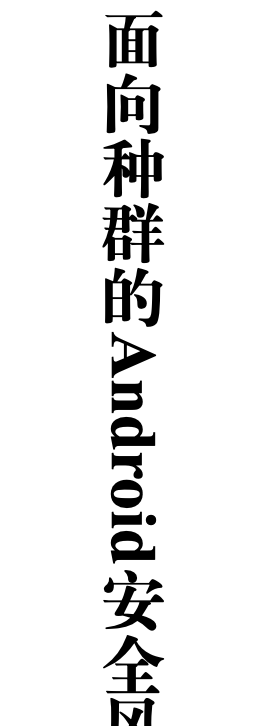
\includegraphics[width=.3\linewidth]{figures/content/2_3}
    \caption{提升基线后的书脊渲染}
    \label{fig:2_3}
    \end{minipage}
\end{figure}

\noindent 这时你必须显式地指定书脊的渲染方式。指定的方式很简单,你只需告知编译引擎对标题中的西文字母进行逆时针270$^{\circ}$(即顺时针90$^{\circ}$)旋转即可:

\begin{tcolorbox}
\begin{lstlisting}[language=TeX]
\spine
    {面向种群的 \rotatebox{270}{Android} 安全风险评估和恶意应用检测}
    {}
\end{lstlisting}
\end{tcolorbox}

\noindent 请注意,{\codefont $\backslash$rotatebox\{270\}\{\}}前后应该各留一个空格,否则会导致编译错误。和论文标题类似,没有副标题时上述第2个字段可以留空。这样修正后的书脊渲染如图 \ref{fig:2_2} 所示。尽管如此,你仍然能从图 \ref{fig:2_2} 中注意到一些异常。拉丁字母在旋转之后的基线高度比汉字基线高度略低,因此导致书脊中的西文部分看起来总是偏左。解决这一问题,你可以在旋转命令中嵌套基线提升命令,就像这样:

\begin{tcolorbox}
\begin{lstlisting}[language=TeX]
\spine
  {面向种群的 \rotatebox{270}{\raisebox{2.5pt}{Android}} 安全风险评估和恶意应用检测}
  {}
\end{lstlisting}
\end{tcolorbox}

再次修正后的书脊渲染如图 \ref{fig:2_3} 所示,这时你就得到了完美的中西文混排书脊。再次强调,如果你的论文标题中没有中西文混排,请直接删去{\codefont $\backslash$spine}字段。

\section{作者与导师}

该部分用于指定论文的作者与导师姓名。作者字段分为2个部分,分别是作者的中文名及其拉丁文转写:

\begin{tcolorbox}
\begin{lstlisting}[language=TeX]
\author
    {陈仁营}
    {CHEN Ren-ying}
\end{lstlisting}
\end{tcolorbox}

\noindent 关于中文姓名转写为英文时的拼写规则,根据《东南大学研究生学位论文格式规定》\cite{seugs2015rule}第一条第二款之要求,有如下规定:

~

\noindent{\color{black!45}
中国姓名译为英文时用汉语拼音,按照姓前名后的原则,姓、名均用全名,不宜用缩写。姓全用大写,名的第一个字母大写,名为双中文字时两个字的拼音之间可以不用短划线,但容易引起歧义时必须用短划线。例如“冯长根”译为“FENG Changgen”或“FENG Chang-gen”,而“冯长安”则必须译为“FENG Chang-an”。论文英文封面上的署名也遵守此规定。}

~

导师字段分为3个部分,分别是导师的中文名、姓名的拉丁文转写以及导师的英文职称,用于显示在英文封面上:

\begin{tcolorbox}
\begin{lstlisting}[language=TeX]
\advisor
    {张广军}
    {ZHANG Guang-Jun}
    {Prof.}
\end{lstlisting}
\end{tcolorbox}

\noindent 对于硕士研究生和博士研究生,导师的职称一般为副教授级及以上。导师为副教授的,职称可以写全称 Associate Professor,也可以写简称 A. Prof.;导师为教授的,可以写全称 Professor或简称Prof.,注意上述简称中的~.不可省略。对于导师职称未达副教授级的特殊情况,比如导师职称为讲师时,请勿在职称处填写Lecturer,此时宜填写Doctor或Dr.以示尊重。

一些硕士研究生可能会有副导师,此时可以显式指定副导师的相关信息,具体方法和导师相同:

\begin{tcolorbox}
\begin{lstlisting}[language=TeX]
\coadvisor
    {程光}
    {CHENG Guang}
    {Prof.}
\end{lstlisting}
\end{tcolorbox}

\noindent 没有副导师的研究生学位论文,请删去上述几行。

\section{答辩信息}

答辩信息用于在论文A3封面和中文彩色封面中渲染与研究生论文答辩相关的信息。

\begin{tcolorbox}
\begin{lstlisting}[language=TeX]
\degreetype{工学硕士}{Master of Engineering}
\major{生物医学工程}
\submajor{神经信息工程}
\defenddate{2020年1月20日}
\authorizedate{2020年1月23日}
\committeechair{齐康}
\reviewer{王建国}{韩冬青}
\department{网络空间安全学院}{School of Cyberspace Security}
\seuthesisthanks{本文的部分工作受国家自然基金 No. wdnmd666 的支持与帮助,在此表示感谢。}
\end{lstlisting}
\end{tcolorbox}

其中,{\codefont degreetype}字段用于指定所申请的学位类型与等级。{\codefont major}和{\codefont submajor}字段用于指定研究生攻读的一级和二级学科名称,请依照中华人民共和国教育部一级和二级学科名录进行填写。如果所属专业直接隶属于一级学科,{\codefont submajor}字段可以留空不填。{\codefont defenddate}和{\codefont authorizedate}分别用于指定论文的答辩日期和学位的授予日期,请根据实际情况填写。{\codefont committeechair}和{\codefont reviewer}用于指定论文的答辩委员会主席和论文评阅人。根据《东南大学研究生学位论文格式规定》\cite{seugs2015rule}第二条第一款之要求,有如下规定:

~

\noindent{\color{black!45}
论文印刷时尚无法填写的评阅人和答辩委员会主席等栏目待答辩完成后要填写补齐,不要空缺。盲审论文的评阅人处标明“盲审”。}

~

{\codefont department}字段用于指定研究生所属的院系,其中院系的英文名将用于英文封面的生成。学院的正确英文译名请查阅所属学院的官方网站。{\codefont seuthesisthanks}用于在论文的中文内页页脚处对论文所属的项目、赞助的基金课题进行简短的鸣谢。此处不宜书写大段文字,请用简单的一两句话对相关组织或机构表示感谢,对其他个人的感谢请在文尾的致谢部分进行。没有相关赞助的学位论文请直接删去该字段。

\section{模板参数}

你有可能已经注意到了在main.tex文件中引入模板类的命令里包含了若干模板参数:

\begin{tcolorbox}
\begin{lstlisting}[language=TeX]
\documentclass[algorithmlist,figurelist,tablelist,nomlist]{seumasterthesis}
\end{lstlisting}
\end{tcolorbox}

\noindent 即{\codefont documentclass}命令后的中括号里的几个参数。这些参数用于控制条件编译以及在论文渲染时向模板类提供额外的信息。本节将会介绍本模板提供的模板参数及其具体含义。

\subsection{链接着色}

本模板通过使用hyperref宏包来提供索引和链接跳转功能。相信你已经注意到了,本模板所渲染出的PDF文档中的所有图片、表格、公式、算法和参考文献索引都被着色高亮,且可以通过点击跳转到原引位置。该功能便于读者在阅读电子文档时快速定位相应索引的位置,但是着色高亮的链接在论文付梓时可能会影响到印刷效果。因此,本模板提供了针对链接着色的模板参数。通过在模板参数列表中添加{\codefont nocolorlinks}参数,模板所渲染出的PDF文档中的所有文献索引都将被取消着色,以便论文的正式印刷。

\subsection{图表、算法及术语目录}

根据不同院系和专业的具体情况,硕士研究生学位论文可能并不需要图表、算法或术语目录中的一项或多项。尽管本模板默认会渲染出上述的所有目录,但是我们也提供了相应的模板参数来灵活控制这些目录的渲染。如果你在模板参数列表中显式指定{\codefont figurelist},代表你希望在论文编译时在章节目录后添加图片目录;类似的,{\codefont tablelist}显式指定了表格目录的需求,{\codefont nomlist}指定了术语表,而{\codefont algorithmlist}指定了算法目录。需要注意的是,你并不需要关注这几个模板参数在参数表中的位置或顺序,具体目录的编译和渲染仍然会依照《东南大学研究生学位论文格式规定》\cite{seugs2015rule}第一条中所规定的顺序进行。

\subsection{硕士类型}

本模板同时支持学术型硕士研究生和专业型硕士研究生。当不添加任何模板参数时,该模板将默认渲染为学术型硕士研究生学位论文;而当在模板参数列表中显式指定{\codefont engineer}时,该模板将渲染为专业型硕士研究生学位论文。专业型与学术型硕士研究生学位论文的区别主要在于以下三点:
\begin{enumerate}
    \item A3 大封面和中文彩色封面的\textbf{标题}。学术型硕士为《硕士学位论文》,专业型硕士为《工程硕士学位论文》。需要注意的是,中文内页封面的标题在两种类型的硕士研究生学位论文中均为《硕士学位论文》。
    \item A3 大封面和中文彩色封面的\textbf{学位论文形式}。专业型硕士研究生需要注明学位论文的研究形式,如应用研究、基础研究或综合研究。因此专业型硕士研究生需要填写main.tex文件中的{\codefont engthesistype}字段,学术型硕士研究生则可以忽略该字段。
    \item A3 大封面和中文彩色封面的\textbf{学科名称}。学术型硕士研究生学位论文需要在答辩信息列表中填写一级和二级学科名称,而专业型硕士研究生需要填写的则是工程领域名称和研究方向。因此专业型硕士研究生需要在main.tex文件的{\codefont major}字段填写自己的工程领域名称,在{\codefont submajor}字段填写自己的研究方向。
\end{enumerate}      % 第二章:
\chapter{撰写正文}

\section{研究生学位论文的一般格式与顺序}

根据《东南大学研究生学位论文格式规定》\cite{seugs2015rule}第一条之要求,研究生学位论文一般应由如下部分组成:

\begin{enumerate}
  \item 中文封面
  \item 中文页面
  \item 英文封面
  \item 论文独创性声明和使用授权声明
  \item 中文内容提要及关键词
  \item 英文内容提要及关键词
  \item 目录
  {\color{cyan} \item 符号、变量、缩略词等本论文专用术语注释表}
  \item 正文
  \item 致谢
  \item 参考文献
  {\color{cyan} \item 附录
  \item 中英文索引
  \item 作者简介(包括在学期间发表的论文和取得的学术成果清单)
  \item 后记}
\end{enumerate}
上述各部分得按照此顺序排列,其中{\color{cyan} 青色}标注的部分为可选部分。我们已经在第\ref{chp:initialization}章中介绍了上述列表中第1-3项关于封面中各条目的填写与生成方法。在本章中,我们将介绍如何撰写论文的正文以及其他部分。

\section{独创性与授权声明}

紧接在中英文封面后的应该是论文的独创性声明和使用授权声明,具体的文本内容请参考《学位论文独创性和使用授权声明》\cite{seugs2018license}。

本模板已经包含了对独创性声明和授权声明的自动生成,当编译引擎执行到

\begin{tcolorbox}
\begin{lstlisting}[language=TeX]
\makebigcover
\makecover
\end{lstlisting}
\end{tcolorbox}

\noindent 时会自动到目录下的seumasterthesis.cfg文件中寻找独创性与授权声明的预定义文本。

\section{中英文摘要}

《东南大学研究生学位论文格式规定》\cite{seugs2015rule}的第一条第二款中对论文摘要有如下要求:

~

{\color{black!45}
\noindent 论文摘要中文约500字左右,英文约200-300词左右,二者应基本对应。它是论文内容的高度概括,应说明研究目的、研究方法、成果和结论,要突出本论文的创造性成果或新的见解,用语简洁、准确。论文摘要后还应注明本文的关键词3-5个。关键词应为公知公用的词和学术术语,不可采用自造字词和略写、符号等,词组不宜过长。

\noindent 英文摘要采用第三人称单数语气介绍该学位论文内容,目的是便于其他文摘摘录,因此在写作英文文摘时不宜用第一人称的语气陈述。叙述的基本时态为一般现在时,确实需要强调过去的事情或者已经完成的行为才使用过去时、完成时等其他时态。可以采用被动语态,但要避免出现用“This paper”作为主语代替作者完成某些研究行为。}

~

打开工程目录下chapters文件夹中的abstract.tex文件,你就可以开始撰写论文的摘要。对于中文摘要,你会看到形如:

\begin{tcolorbox}
\begin{lstlisting}[language=TeX]
\begin{abstract}{生物学, 钓鱼, 铁憨憨}
我今天没吃饱。下面我将用70页的篇幅说明我今天为啥没吃饱,但是你看完后不一定能看懂。
\end{abstract}
\end{lstlisting}
\end{tcolorbox}

\noindent 这样的结构。在{\codefont $\backslash$begin\{abstract\}}之后的大括号里,你可以填写你的中文关键词。接下来直到{\codefont $\backslash$end\{abstract\}}之前的所有内容都将在编译时被视作你中文摘要的正文内容。英文摘要也与此类似,在abstract.tex文件中,你会看到形如:

\begin{tcolorbox}
\begin{lstlisting}[language=TeX]
\begin{englishabstract}{Biology, Phishing, Fucking Idiot}
I am not full today. I will use 70 pages to explain why I ain't full, but you may not understand after reading this piece of shit.
\end{englishabstract}
\end{lstlisting}
\end{tcolorbox}

\noindent 这样的结构,你可以把你的英文关键词和摘要填写在相应的位置。main.tex主文件通过:

\begin{tcolorbox}
\begin{lstlisting}[language=TeX]
%% ----------------------------------------------------------------------------
%%                              Chinese Abstract
%% ----------------------------------------------------------------------------
\begin{abstract}{\TeX, \LaTeX, 学位论文}
本文提出了一个新的东南大学 \LaTeX 硕士研究生毕业论文模板,并说明了如何更优雅地写出一篇漂亮而无用的文章。
\end{abstract}

%% ----------------------------------------------------------------------------
%%                              English Abstract
%% ----------------------------------------------------------------------------
\begin{englishabstract}{\TeX, \LaTeX, Thesis}
This article proposes a new Southeast University master degree thesis \LaTeX ~template and explains how to elegantly write an article which is beautiful but full of shit.
\end{englishabstract}

\end{lstlisting}
\end{tcolorbox}

\noindent 将abstract.tex文件作为外部依赖引入到主文件中,编译引擎在执行到该语句时会自动到chapters目录下寻找相应文本。

\section{论文章节及图表目录}
\label{sec:content}

本模板支持对所有章节和图表自动生成目录,在main.tex中:

\begin{tcolorbox}
\begin{lstlisting}[language=TeX]
\tableofcontents
\listofothers
\end{lstlisting}
\end{tcolorbox}

\noindent 语句控制了所有目录的自动生成,你不需要进行任何多余的操作。

\section{正文}
\label{sec:main_body}

我们在chapters目录下为你准备了若干名为chapterx.tex的文件,我们建议你将正文分章节书写在这些文件中。如果我们为你准备的6个章节文件尚且不能够满足你的章节数量需求,你可以继续在该目录下创建新的章节文件,并将其作为外部依赖添加到main.tex主文件中,就像这样:

\begin{tcolorbox}
\begin{lstlisting}[language=TeX]
...
\chapter{版权信息与更新记录}
\label{chp:version_license}

\section{版权信息}

本模板基于宋睿同学发布在\href{https://github.com/TouchFishPioneer/SEU-master-thesis}{SEU-master-thesis} 并在上述工作的基础上进行了微调,解决了一些自己编写代码过程中 BUG。
\input{chapters/chapter7}
\input{chapters/chapter8}
...
\end{lstlisting}
\end{tcolorbox}

本模板对文章的章节结构支持到了小节级别。如果你想创建新的章,请使用:

\begin{tcolorbox}
\begin{lstlisting}[language=TeX]
\chapter{母猪的产后护理}
\end{lstlisting}
\end{tcolorbox}

\noindent 这样的命令,它将为你新建一个名为“母猪的产后护理”的章。节与小节的创建方法与此类似:

\begin{tcolorbox}
\begin{lstlisting}[language=TeX]
\section{母猪产后抑郁了怎么办}
\subsection{母猪的心理疏导}
\end{lstlisting}
\end{tcolorbox}

\LaTeX 相比于Microsoft Word等文本编辑器的优势在于,它对交叉引用和自动编号的支持极其自然和友好,以至于你完全不需要耗费精力管理相关的内容。比如说你在正文中需要引用前文的某个章节,你只需要在该章节处添加一个标签,就像这样:

\begin{tcolorbox}
\begin{lstlisting}[language=TeX]
\chapter{母猪的产后护理}
\label{chp:postnatal_care}
\end{lstlisting}
\end{tcolorbox}

\noindent 随后如果你想要在其他部分引述该章节的内容。你只需要在相应位置插入该章节的标签,就像这样:

\begin{tcolorbox}
\begin{lstlisting}[language=TeX]
在第\ref{chp:postnatal_care}章,我们介绍了如何对母猪进行产后护理。那么萨达姆是如何根据该经验做好对美国的战斗准备的呢?
\end{lstlisting}
\end{tcolorbox}

\noindent 那么在论文编译时,上面的引用就会被自动替换为相应章节的名称,就像这样:

\begin{tcolorbox}
\begin{lstlisting}[language=TeX]
在第三章,我们介绍了如何对母猪进行产后护理。那么萨达姆是如何根据该经验做好对美国的战斗准备的呢?
\end{lstlisting}
\end{tcolorbox}

\noindent 在论文的撰写过程中请活用该功能,它能为你提供许多方便。

\section{致谢}

你可以在chapters目录下的acknowledgement.tex文件中写下你对任何人的任何感谢,这是学位论文中你唯一可以恣情释放的地方,请尽情享受吧。

\section{参考文献}

和目录与引用类似,本模板支持对参考文献列表的自动生成,在main.tex中:

\begin{tcolorbox}
\begin{lstlisting}[language=TeX]
\thesisbib{seumasterthesis}
\end{lstlisting}
\end{tcolorbox}

\noindent 命令实现了这一功能。关于如何引入参考文献以及如何在正文中引用特定的参考文献条目,我们还将在第\ref{chp:bib}章进行详细地介绍。

\section{附录}

根据《东南大学研究生学位论文格式规定》\cite{seugs2015rule}的第一条第八款,你可以将正文有关的原始数据明细表、较多的图表、程序源代码、过长的公式推导等不宜置于正文部分的文本放在附录中。你可以在chapters目录下的appendix.tex文件中添加你的附录。如果你有多个附录的话,可以通过在该文件中新增:

\begin{tcolorbox}
\begin{lstlisting}[language=TeX]
\chapter{沙漠风暴行动D日攻击计划表}
\end{lstlisting}
\end{tcolorbox}

\noindent 来添加附录项。每个附录项都将被以大写英文字母编号和排序,并均会新起一页。除此之外,附录内容的撰写方法和正文基本一致。

如果你的论文不需要安排附录,请在main.tex主文件中删去或注释该行:

\begin{tcolorbox}
\begin{lstlisting}[language=TeX]
\appendix
\newtheorem{theorem}{定理}

\chapter{欧几里得第二定理的证明}
\label{appendix:apps}

	\begin{theorem}
		欧几里得第二定理(素数有无穷多个)\\
		证明:用反证法。假设素数有有限个($N$个),记为$p_1,p_2,\dots,p_N$。则我们构造一个新的数,
		
		\[n=p_1p_2\dots p_N+1.\]
		
		由于$p_i,i=1,2,\dots,N$为素数,则一定不为$1$。于是对于任意的$p_i,i=1,2,\dots, N$,有
		
		\[p_i\not|n\]
		
		这表明,要么$n$本身为素数,要么$n$为合数,但是存在$p_1,p_2,\dots,p_N$之外的其他素数能够将$n$进行素因子分解。不管哪种情况,都表明存在更多的素数。定理得证。\qed
	\end{theorem}

\chapter{$\sqrt{2}$是无理数的证明}
	\begin{theorem}
		$\sqrt{2}$是无理数。\\
		证明:用反证法。假设$\sqrt{2}$是有理数,则可表示为两个整数的商,即$\exists p,q, q\ne0$
		
		\[\sqrt{2}=\frac{p}{q}\]
		
		不失一般性,我们假设$p,q$是既约的,即$\gcd(p,q)=1$。对上式两边平方可得\\
		
		\begin{align*}
			2& =\frac{p^2}{q^2}\\
			p^2&=2q^2.
		\end{align*}
		
		表明$p^2$为偶数,因此$p$为偶数,记$p=2m$。则
		
		\begin{align*}
			p^2&=4m^2=2q^2\\
			q^2&=2m^2.
		\end{align*}
		
		表明$q$也为偶数,因此它们有公共因子$2$。这与它们既约的假设矛盾。定理得证。\qed
	\end{theorem} 
\end{lstlisting}
\end{tcolorbox}

\section{作者简介}

你可以在作者简介部分简要介绍你的姓名、出生年月、籍贯等基本信息,并简要列举你在攻读学位阶段参与的科研课题、发表的学术论文、获取的发明专利或著作权,以及其他的一些科研成果。《东南大学研究生学位论文格式规定》\cite{seugs2015rule}的第一条第十款建议硕士研究生将该部分限制在1000字以内,博士研究生则在2000字以内。

我们在chapters目录下的resume.tex文件中为你准备了一份模板,你可以根据你的实际情况进行修改。      % 第三章:
\chapter{特殊环境与浮动体}
\label{chp:float}

事实上我们本该假设所有使用本 \LaTeX 论文模板的人都具备了相当的 \LaTeX 使用经验和知识,如果这样那么本章所介绍的内容是不言自明的。但是也存在很多初次接触 \LaTeX 的研究生朋友,因为各种不同的原因而尝试使用 \LaTeX 进行论文排版。因此我们认为还是有必要对这些 \LaTeX 中的基本元素进行反复地强调,以避免我们的个别开发者的邮箱和GitHub Issues被投诉和问询填满。如果你是一个 \LaTeX 老手,你可以直接跳过本章而不用担心漏过任何重要内容。

\section{图片}

\subsection{插入图片}
在 \LaTeX 文档中插入图片,你需要如下的代码:

\begin{tcolorbox}
\begin{lstlisting}[language=TeX]
\begin{figure}[htbp]
  \centering
  
\includegraphics[width=.3\linewidth]{figures/content/4_1}
  \caption{插入图片示例}
  \label{fig:4_1}
\end{figure}
\end{lstlisting}
\end{tcolorbox}

\noindent 上面的代码会插入如下效果的图片:

\begin{figure}[htbp]
  \centering
  
\includegraphics[width=.3\linewidth]{figures/content/4_1}
  \caption{插入图片示例}
  \label{fig:4_1}
\end{figure}

\subsection{浮动体环境与位置标识符}

\begin{tcolorbox}
\begin{lstlisting}[language=TeX]
\begin{figure}[htbp]
\end{figure}
\end{lstlisting}
\end{tcolorbox}

\noindent 声明了一个图片浮动体环境。浮动体是 \LaTeX 中的一种特殊容器,用于容纳占据篇幅较大但不方便分页的内容,如图片或表格。方括号中的字母是浮动体位置标识符,用于向 \LaTeX 编译引擎提出位置建议。常见的位置标识符有以下4种:

\begin{itemize}
  \setlength{\itemsep}{1.5pt}
  \setlength{\parsep}{1.5pt}
  \setlength{\parskip}{1.5pt}
  \item {\codefont h}:表示here。\LaTeX 编译引擎在面对用{\codefont h}标识的浮动体时会首先尝试在声明位置插入浮动体;
  \item {\codefont t}:表示top。\LaTeX 编译引擎会尝试在当页顶部安置浮动体;
  \item {\codefont b}:表示bottom。\LaTeX 编译引擎会尝试在当页底部安置浮动体;
  \item {\codefont p}:表示float page。\LaTeX 编译引擎会尝试为该浮动体分页并使其占据全页。
\end{itemize}

你可以使用多个位置标识符并将其自由组合,你指定的顺序代表你向 \LaTeX 编译引擎所推荐的优先级。需要说明的是,编译引擎并不保证会按照你所指定的位置优先级安置浮动体,而是会根据浮动体大小、其在页面中的位置、文字的相对分布等多种因素决定浮动体的位置。因此在论文写作过程中,我们不建议你使用如“下图”,“上表”等使用方位来指代特定图片或表格的表述,因为你所插入的图片或表格很有可能并不会被编译到你想要它出现的位置。当然,你也可以在标识符前加上 !号来表示强制位置,如{\codefont !h}。但是我们不推荐这样做,因为这可能会造成很多你意想不到的后果。

来自 Reanon的建议: 一般情况下使用「htbp」就够了。有时候图片表格过大,导致它们出现独占一页的情况,可以使用 「H」来强制指定位置。

\subsection{图片的大小与路径}

\begin{tcolorbox}
\begin{lstlisting}[language=TeX]
\centering

\includegraphics[width=.5\linewidth]{figures/content/4_1}
\end{lstlisting}
\end{tcolorbox}

{\codefont centering}表示浮动体在控制范围内居中。{\codefont includegraphics}语句向编译引擎指定你所想要引入的图片的大小与保存路径。在该命令之后跟随的方括号中,你可以指定图片的长或宽。默认情况下 \LaTeX 会锁定图片的长宽比例,因此你只需要指定长宽中的一个即可。后面的大括号用于填写图片的路径,你可以使用主文件main.tex的相对路径来表示。我们在模板根目录下设置了一个名为figures的目录用于存放图片,我们建议你把论文需要的所有图片放置于该目录下的content文件夹中以便查找和管理。

\subsection{图片的标题与标签}

\begin{tcolorbox}
\begin{lstlisting}[language=TeX]
\caption{插入图片示例}
\label{fig:4_1}
\end{lstlisting}
\end{tcolorbox}

{\codefont caption}用于指定图片的标题。{\codefont label}用于给图片添加标签,便于你在文本中引用该图片。对于上面的图片,如果我们想要在论文中引述其内容,可以采用如下方法:

\begin{tcolorbox}
\begin{lstlisting}[language=TeX]
图\ref{fig:4_1}是东南大学的校徽,它的设计中蕴含着多种寓意。
\end{lstlisting}
\end{tcolorbox}

\noindent 上述文本在编译后会呈现这样的效果:

图\ref{fig:4_1}是东南大学的校徽,它的设计中蕴含着多种寓意。

\subsection{图片的并排}

很多时候,你可能会想要将两张图片并排放置以节省排版空间。我们支持并鼓励你这样做。你只需要引入如下的代码:

\begin{tcolorbox}
\begin{lstlisting}[language=TeX]
\begin{figure}[htbp]
  \centering
    \begin{minipage}[t]{0.48\textwidth}
      \centering
      
\includegraphics[width=6cm]{figures/content/4_2}
      \caption{GitHub}
      \label{fig:4_2}
    \end{minipage}
    \begin{minipage}[t]{0.48\textwidth}
      \centering
      
\includegraphics[width=8cm]{figures/content/4_3}
      \caption{NPM}
      \label{fig:4_3}
    \end{minipage}
\end{figure}
\end{lstlisting}
\end{tcolorbox}

\noindent 编译后的效果是这样的:

\begin{figure}[htbp]
  \centering
    \begin{minipage}[t]{0.48\textwidth}
      \centering
      
\includegraphics[width=4cm]{figures/content/4_2}
      \caption{GitHub}
      \label{fig:4_2}
    \end{minipage}
    \begin{minipage}[t]{0.48\textwidth}
      \centering
      
\includegraphics[width=3cm]{figures/content/4_3}
      \caption{npm}
      \label{fig:4_3}
    \end{minipage}
\end{figure}

注意,在上述代码中,我们定义了一个{\codefont figure}浮动体环境,并在其中用两个:

\begin{tcolorbox}
\begin{lstlisting}[language=TeX]
\begin{minipage}[t]{0.48\textwidth}
\end{minipage}
\end{lstlisting}
\end{tcolorbox}

\noindent 包裹了两张图片的声明。和单个图片类似,你也可以指定{\codefont minipage}相对浮动体的位置和大小。编译引擎将根据你{\codefont minipage}的大小调整在一行显示的图片数量。需要注意的是,在两个{\codefont minipage}声明之间请勿空行,因为 \LaTeX 编译引擎会将空行视作换行请求而错误地将你的两张图片上下放置。

\subsection{子图}

和图片并排类似,子图也用于提供在水平方向上组织浮动体的功能。和图片的简单并排不同的是,子图功能一般用于表达同一主题下内容相近或有对比意义的图片或其他浮动体。对于子图功能,你需要引入如下代码:

\begin{tcolorbox}
\begin{lstlisting}[language=TeX]
\begin{figure}[htbp]
  \centering
  \subfloat[彩色标志]{
\includegraphics[width=.38\textwidth]{figures/content/4_4}}
  \quad\quad
  \subfloat[单色标志]{
\includegraphics[width=.38\textwidth]{figures/content/4_5}}
  \caption{东南大学校徽的视觉设计}
  \label{fig:4_4}
\end{figure}
\end{lstlisting}
\end{tcolorbox}

\noindent 编译后呈现如下效果:

\begin{figure}[htbp]
  \centering
  \subfloat[彩色标志]{
\includegraphics[width=.38\textwidth]{figures/content/4_4}}
  \quad\quad
  \subfloat[单色标志]{
\includegraphics[width=.38\textwidth]{figures/content/4_5}}
  \caption{东南大学校徽的视觉设计}
  \label{fig:4_4}
\end{figure}

\noindent {\codefont subfloat}命令指定了图片的子图单元,你可以在命令后的方括号中指定子图的名称,并在随后的大括号中声明子图的版式和索引路径。

\section{表格}

\subsection{插入表格}

在论文中插入表格的方法与图片类似,示例代码如下:

\begin{tcolorbox}
\begin{lstlisting}[language=TeX]
\begin{table}[htbp]
\centering
\caption{东南大学院系列表}
\label{tab:4_1}
\begin{tabular}{cll}
\toprule
院系编号&\multicolumn{1}{c}{院系名称}&\multicolumn{1}{c}{院系英文译名}\\
\midrule
01  & 建筑学院      & School of Architecture  \\
02  & 机械工程学院    & School of Mechanical Engineering \\
03  & 能源与环境学院   & School of Energy and Environment \\
04  & 信息科学与工程学院 & School of Information Science and Engineering \\
05  & 土木工程学院    & School of Civil Engineering \\
\bottomrule
\end{tabular}
\end{table}
\end{lstlisting}
\end{tcolorbox}

\noindent 编译后的效果如表 \ref{tab:4_1} 所示。

\begin{table}[htbp]
\centering
\caption{东南大学院系列表}
\label{tab:4_1}
\begin{tabular}{cll}
\toprule
院系编号 & \multicolumn{1}{c}{院系名称}       & \multicolumn{1}{c}{院系英文译名 }     \\
\midrule
01                       & 建筑学院      & School of Architecture                        \\
02                       & 机械工程学院    & School of Mechanical Engineering              \\
03                       & 能源与环境学院   & School of Energy and Environment              \\
04                       & 信息科学与工程学院 & School of Information Science and Engineering \\
05                       & 土木工程学院    & School of Civil Engineering \\
\bottomrule
\end{tabular}
\end{table}

\noindent 想要定义一个表格,首先需要声明浮动体环境:

\begin{tcolorbox}
\begin{lstlisting}[language=TeX]
\begin{table}[htbp]
  \centering
  \caption{东南大学院系表}
  \label{tab:4_1}
\end{table}
\end{lstlisting}
\end{tcolorbox}

\noindent 在声明表格浮动体时,你也可以指定该表格的标题和标签,这与图片的声明类似。需要提醒的是,根据《东南大学研究生学位论文格式规定》\cite{seugs2015rule}第一条第五款第六则的要求,表格的标题应该位于表格的上方,而图片的标题应该出现在图片的下方。

表格的具体内容在需要在浮动体中用{\codefont tabular}环境声明:

\begin{tcolorbox}
\begin{lstlisting}[language=TeX]
\begin{tabular}{cll}
  \toprule
  院系编号&\multicolumn{1}{c}{院系名称}&\multicolumn{1}{c}{院系英文译名}\\
  \midrule
  01  & 建筑学院      & School of Architecture  \\
  02  & 机械工程学院    & School of Mechanical Engineering \\
  03  & 能源与环境学院   & School of Energy and Environment \\
  04  & 信息科学与工程学院 & School of Information Science and Engineering \\
  05  & 土木工程学院    & School of Civil Engineering \\
  \bottomrule
\end{tabular}
\end{lstlisting}
\end{tcolorbox}

\noindent {\codefont tabular}声明后面紧跟着的是表格的纵向对其标准,比如我们的表格有3列,就需要使用3个字母分别指定这3列的对齐准则。你可以使用{\codefont l}表示左对齐,使用{\codefont r}表示右对齐,而使用{\codefont c}表示居中。下面你就可以以行为单位添加表格的内容,行与行间用两条反斜杠隔开,而行中的不同列间使用符号\&隔开。

需要特别注意的是,学术论文一般要求所有表格采用三线表形式。对于三线表,其列间不允许存在竖分割线,而行间仅在表顶、表头与表身、表尾处用三条横线确定表格的结构。因此在表格绘制时,你需要手动指定三线的位置,并在相应的行间添加下面三条指令,分别指代顶线、中间线和尾线:

\begin{tcolorbox}
\begin{lstlisting}[language=TeX]
\toprule
\midrule
\bottomrule
\end{lstlisting}
\end{tcolorbox}

事实上,在 \LaTeX 文本中插入表格确实需要付出很大的精力对表格的内容和样式进行调整,这也是很多初学者诟病 \LaTeX 的原因之一。为了方便你设计表格,我们向你推荐\href{http://www.tablesgenerator.com/}{一个网站},该网站能够使用图形化界面创建表格,然后自动生成对应的 \LaTeX 代码。你只需要把代码复制到你的文档中,并稍加调整与修正即可。

\section{算法}

一些理学和工学专业的研究可能需要在论文中插入为代码或算法,本模板同样支持这一功能。示例代码如下:

\begin{tcolorbox}
\begin{lstlisting}[language=TeX]
\begin{algorithm}
\caption{辗转相除法}
\label{alg:4_1}
\begin{algorithmic}[1]
\Require 一个整数$m$
\Require 另一个整数$n$
\Ensure $m$和$n$的最大公约数$r$
\While {$n > 0$}
    \State $t \leftarrow m ~ mod ~ n$
    \State $m \leftarrow n$
    \State $n \leftarrow t$
\EndWhile
\State $r \leftarrow t$
\end{algorithmic}
\end{algorithm}
\end{lstlisting}
\end{tcolorbox}

\noindent 上述代码的编译结果如算法 \ref{alg:4_1} 所示。

\begin{algorithm}
\caption{辗转相除法}
\label{alg:4_1}
\begin{algorithmic}[1]
\Require 一个整数$m$
\Require 另一个整数$n$
\Ensure $m$和$n$的最大公约数$r$
\While {$n > 0$}
    \State $t \leftarrow m ~ mod ~ n$
    \State $m \leftarrow n$
    \State $n \leftarrow t$
\EndWhile
\State $r \leftarrow t$
\end{algorithmic}
\end{algorithm}

和图片和表格类似,声明算法之前你首先要声明用于安放算法伪代码的浮动体:

\begin{tcolorbox}
\begin{lstlisting}[language=TeX]
\begin{algorithm}
  \caption{辗转相除法}
  \label{alg:4_1}
\end{algorithm}
\end{lstlisting}
\end{tcolorbox}

\noindent 随后使用{\codefont algorithmic}开始添加你的伪代码的具体内容。在这里由于篇幅所限,我们仅会提示一些{\codefont algorithmic}最简单的用法。对于算法的输入项,你需要使用{\codefont $\backslash$Require}命令指明,而输出项使用{\codefont $\backslash$Ensure}命令。对于声明和赋值语句,请你以{\codefont $\backslash$State}开头,而对于判断、循环语句,应该使用如下的形式表达:

\begin{tcolorbox}
\begin{lstlisting}[language=TeX]
\If \EndIf
\While \EndWhile
\For \EndFor
\end{lstlisting}
\end{tcolorbox}

\noindent 请注意,这些语句必须两两配对,否则编译时会出现错误。想要了解更多{\codefont algorithmic}的用法和范例,请自行百度或者参考其官方文档。

来自 Reanon 的建议:「$\backslash$begin{algorithmic}[1]」可以显示算法的行号

\section{公式环境}

很多时候,你的论文可能会涉及公式和逻辑推导,这时你可能需要插入数学公式环境。\LaTeX 中的数学公式分为两种,分别是行内公式和行间公式环境。当你想要在文本叙述中插入数学符号时,你需要的是行内公式。你只需要用两个\$符号包裹你的数学符号即可,就像这样:

\begin{tcolorbox}
\begin{lstlisting}[language=TeX]
对于$\forall \theta \in \Theta$,如果有$\theta$使得...
\end{lstlisting}
\end{tcolorbox}

\noindent 编译后的结果是这个样子的:

对于$\forall \theta \in \Theta$,如果有$\alpha$使得...

但是当你想要表达数学逻辑的推导或者方程的计算时,你可能需要整块行间的区域进行系统性地阐述,这时你需要使用行间公式环境。就像这样:

\begin{tcolorbox}
\begin{lstlisting}[language=TeX]
\begin{equation}
  \label{eq:4_1}
  f(x) = \frac{f(x_0)}{0!} + \frac{f'(x_0)}{1!}(x-x_0) + \dots + \frac{f^{(0)}(x_0)}{n!}(x-x_0)^n + R_n(x)
\end{equation}
\end{lstlisting}
\end{tcolorbox}

\noindent 上述代码编译后将呈现这样的效果:

\begin{equation}
  \label{eq:4_1}
  f(x) = \frac{f(x_0)}{0!} + \frac{f'(x_0)}{1!}(x-x_0) + \dots + \frac{f^{(0)}(x_0)}{n!}(x-x_0)^n + R_n(x)
\end{equation}

\noindent 公式 \ref{eq:4_1} 展示了单行行间公式的表达方式。有时候你还可能需要展示多行的公式,并且这些公式还要按照某些方式对齐。这时候你需要在{\codefont equation}环境中再嵌套一个{\codefont aligned}环境。在每行需要对齐的部分,你可以使用{\codefont \&}符号显式地指明,就像这样:

\begin{tcolorbox}
\begin{lstlisting}[language=TeX]
\begin{equation}
  \label{eq:4_2}
  \begin{aligned}
  \int_{-\infty}^{\infty}f(x)dx & = \frac{1}{2\lambda}\int_{-\infty}^{\infty}e^{-\frac{|x-\mu|}{\lambda}}dx \\
  & = \frac{1}{2}\int_{-\infty}^{\infty}e^{-|t|}dt \\
  & = 1
  \end{aligned}
\end{equation}
\end{lstlisting}
\end{tcolorbox}

\noindent 上述代码编译后将呈现这样的效果:

\begin{equation}
  \label{eq:4_2}
  \begin{aligned}
  \int_{-\infty}^{\infty}f(x)dx & = \frac{1}{2\lambda}\int_{-\infty}^{\infty}e^{-\frac{|x-\mu|}{\lambda}}dx \\
  & = \frac{1}{2}\int_{-\infty}^{\infty}e^{-|t|}dt \\
  & = 1
  \end{aligned}
\end{equation}

我们只展示了一小部分数学公式的语法,如果你有更复杂的表达需求,请自行百度。

\section{引用浮动体}

我们已经在 \ref{sec:main_body} 节中介绍了正文章节的引用,并在本章展示了对图、表、算法和公式的引用。为了使你在面临大量标签时也能够快速找到你需要引用的内容,同时也为了提升你文档的结构与条理,我们建议你分别用不同的前缀表记不同类型的引用对象,就像这样:

\begin{tcolorbox}
\begin{lstlisting}[language=TeX]
\label{chp:chapter_name}
\label{sec:section_name}
\label{subsec:subsection_name}
\label{fig:figure_name}
\label{tab:table_name}
\label{alg:algorithm_name}
\label{eq:equation_name}
\end{lstlisting}
\end{tcolorbox}

\noindent 你也可以设计你自己的引用标签,上面的示例只是我们的一个建议。很多编辑器在你输入{\codefont ref}时会自动弹出代码提示,自定义标签配合代码提示能够帮助你更快索引到你想要的引用标签。

\section{代码环境}

一些计算机、软件、电子等专业的毕业论文可能需要展示少量代码,本模板同样也提供了代码环境。比如,下面我们展示了一个Java程序:

\begin{tcolorbox}
\begin{lstlisting}[language=Java]
public static void main(String[] args) {
    System.out.println("你好世界");
}
\end{lstlisting}
\end{tcolorbox}

想要实现这样的效果,你只需要将代码包裹在{\codefont lstlisting}环境中。你还可以指定代码所属的语言,这样{\codefont lstlisting}环境就可以为你实现一定程度上的代码高亮。想要查询你所使用的计算机语言是否被{\codefont lstlisting}支持,请直接参阅{\codefont lstlisting}的官方文档。

\section{术语与符号}

你的论文中可能涉及到了大量的符号、英文缩写或术语,你可以在文中对这些符号进行说明,就像这样:

\begin{tcolorbox}
\begin{lstlisting}[language=TeX]
\nomenclature{PDF}{Portable Document Format}
\end{lstlisting}
\end{tcolorbox}

\noindent 你应该在{\codefont nomenclature}命令后的第一对括号中填写术语或符号名称,下一对括号中填写对术语或符号的解释或定义。当论文编译时,这些术语与符号将会被自动列入目录页后的术语与符号表,并按照英文字母序排列。      % 第四章:
\chapter{参考文献}
\label{chp:bib}

\section{导入参考文献}

你有多种方式导入参考文献,最常用的一种是直接从百度学术或谷歌学术中获取文献的 BibTeX 信息,就像这样:

\begin{tcolorbox}
\begin{lstlisting}[language=TeX]
@article{blum2013learning,
  title={A learning theory approach to noninteractive database privacy},
  author={Blum, Avrim and Ligett, Katrina and Roth, Aaron},
  journal={Journal of the ACM (JACM)},
  volume={60},
  number={2},
  pages={1--25},
  year={2013},
  publisher={ACM New York, NY, USA}
}
\end{lstlisting}
\end{tcolorbox}

你只需要将其粘贴到模板根目录下的seumasterthesis.bib文件中,就能够在你的论文中引用该文献。

\section{引用参考文献}

在你的正文中,你有两种方法引用参考文献,其中一种是这样的:

\begin{tcolorbox}
\begin{lstlisting}[language=TeX]
\cite{blum2013learning}
\end{lstlisting}
\end{tcolorbox}

\noindent 它用于实现上标样式的文献引用,就像这样\cite{blum2013learning}。一般我们引用参考文献均采用这种方式。而在另一些情况下,你所引用的参考文献需要在文章或段落中充当语言成分,这时你应当这样引用参考文献:

\begin{tcolorbox}
\begin{lstlisting}[language=TeX]
\citen{blum2013learning}
\end{lstlisting}
\end{tcolorbox}

\noindent 比如在文献综述中,你可能需要这样列举文章所做的工作:

文章\citen{blum2013learning}提出了一种基于非交互式数据库隐私的机器学习理论...

\section{参考文献样式}

本模板的参考文献渲染样式基于GB/T 7714-2015国家标准,模板的BST文件来自南京大学的\href{https://github.com/Haixing-Hu}{胡海星}同学提供的\href{https://github.com/CTeX-org/gbt7714-bibtex-style}{CTeX-org},在此对他的工作表示感谢。

此外,工程根目录下的附录3是《中华人民共和国关于参考文献著录规则的国家标准 GB/T 7714-2015》的原文,有需要的同学可以参阅。      % 第五章:
\chapter{版权信息与更新记录}
\label{chp:version_license}

\section{版权信息}

本模板基于宋睿同学发布在\href{https://github.com/TouchFishPioneer/SEU-master-thesis}{SEU-master-thesis} 并在上述工作的基础上进行了微调,解决了一些自己编写代码过程中 BUG。      % 第六章:

%% ----------------------------------------------------------------------------
%%            Acknowledgement, Appendix, Bibliography and Resume
%% ----------------------------------------------------------------------------
\acknowledgement
感谢许元和樊智猛等前人的工作,没有他们的工作也就不会有这个模板的诞生。也感谢使用该模板的每一个人,因为你们的开放与进取心使得 \LaTeX 在东南大学的氛围越来越好。    % 致谢
\thesisbib{IEEEfull,reference}               % 生成参考文献

%% 下面一句只是用于提示 TexPad 参考文献位置,正式生成时一定要删除
% \bibliography{reference.bib} % 告诉编译器参考文献所在文件

\appendix
\newtheorem{theorem}{定理}

\chapter{欧几里得第二定理的证明}
\label{appendix:apps}

	\begin{theorem}
		欧几里得第二定理(素数有无穷多个)\\
		证明:用反证法。假设素数有有限个($N$个),记为$p_1,p_2,\dots,p_N$。则我们构造一个新的数,
		
		\[n=p_1p_2\dots p_N+1.\]
		
		由于$p_i,i=1,2,\dots,N$为素数,则一定不为$1$。于是对于任意的$p_i,i=1,2,\dots, N$,有
		
		\[p_i\not|n\]
		
		这表明,要么$n$本身为素数,要么$n$为合数,但是存在$p_1,p_2,\dots,p_N$之外的其他素数能够将$n$进行素因子分解。不管哪种情况,都表明存在更多的素数。定理得证。\qed
	\end{theorem}

\chapter{$\sqrt{2}$是无理数的证明}
	\begin{theorem}
		$\sqrt{2}$是无理数。\\
		证明:用反证法。假设$\sqrt{2}$是有理数,则可表示为两个整数的商,即$\exists p,q, q\ne0$
		
		\[\sqrt{2}=\frac{p}{q}\]
		
		不失一般性,我们假设$p,q$是既约的,即$\gcd(p,q)=1$。对上式两边平方可得\\
		
		\begin{align*}
			2& =\frac{p^2}{q^2}\\
			p^2&=2q^2.
		\end{align*}
		
		表明$p^2$为偶数,因此$p$为偶数,记$p=2m$。则
		
		\begin{align*}
			p^2&=4m^2=2q^2\\
			q^2&=2m^2.
		\end{align*}
		
		表明$q$也为偶数,因此它们有公共因子$2$。这与它们既约的假设矛盾。定理得证。\qed
	\end{theorem}            % 附录
\resume{作者攻读硕士学位期间的研究成果}

% 知心哥哥(1996.3.3 -),男,台湾南昌人,现居台湾重庆,为网易CC丢人主播,主要研究方向有《黑旗》、《黑楼》和《黑暗剑》。

~~

\begin{flushleft} 
  \bfseries\large 论文\\
  \relax
\end{flushleft}

\begin{enumerate}
  \renewcommand{\labelenumi}{[\theenumi]}
  \item \textbf{ZHi X}, WEI T, CHEN R, et al. Sea of Thieves: Fucking Animal[C]. 2017 810th International Conference on Disgraced (ICD). Chongqing, 2017. 1-6. (EI Indexed)
  \item \textbf{ZHi X}, WEI T, JI H, et al. Animal Crossing: Playing Together[J]. Nintendo Daily Journal, 2020, 13(3): 114-514. (SCI Indexed)
  \item 韦天, \textbf{知心哥哥}. 你怪猎来我大圣:3D游戏之耻[C]. 第19届口吐芬芳游戏评测国际会议(SFGR). 台湾南昌, 2019. 1-14. (EI Indexed)
\end{enumerate}

~~

\begin{flushleft}
  \bfseries\large 科研项目\\
  \relax
\end{flushleft}

\begin{enumerate}
  \renewcommand{\labelenumi}{[\theenumi]}
  \item \textbf{2018.5-2019.2}:底特律便乘人暨强人工智能的实现
  \item \textbf{2020.1-2020.3}:大老爹拿球的概率模型研究
\end{enumerate}
             % 作者简介
\clearpage
\thispagestyle{empty}
\begin{center}
    \xiaoerhao\songti\bfseries 毕业/学位论文答辩委员会名单
\end{center}
% Please add the following required packages to your document preamble:
% \usepackage{multirow}
\begin{table}[h]
\renewcommand\arraystretch{1.3}
\centering
\begin{tabular}{|cc|ccc|}
\hline
\multicolumn{2}{|c|}{\textbf{毕业/学位论文题目}}    & \multicolumn{3}{l|}{东南大学 LATEX 论文模板使用手册}  \\ \hline
\multicolumn{2}{|c|}{\textbf{作  者}} & \multicolumn{3}{l|}{XXX} \\ \hline
\multicolumn{2}{|c|}{\textbf{专  业}} & \multicolumn{3}{l|}{通信工程(含宽带网络、移动通信)等}        \\ \hline
\multicolumn{2}{|c|}{\textbf{研究方向}} & \multicolumn{3}{l|}{通信与信息系统}\\ \hline
\multicolumn{2}{|c|}{\textbf{导  师}} & \multicolumn{3}{l|}{XXX}  \\ \hline
\multicolumn{1}{|c|}{\multirow{7}{*}{\bfseries \parbox[t]{1em}{答辩委员会组成}}} & \textbf{姓  名}   & \multicolumn{1}{c|}{\textbf{职  称}}        & \multicolumn{1}{c|}{\textbf{学科专业}} & \textbf{工作单位} \\ \cline{2-5} 
\multicolumn{1}{|c|}{}    & \multicolumn{1}{c|}{\renewcommand\arraystretch{1}\begin{tabular}[c]{@{}c@{}}XXX\\ (主席)\end{tabular}} & \multicolumn{1}{c|}{研究员}  & \multicolumn{1}{c|}{ 信息与通信工程 }       & XX大学\\ \cline{2-5} 
\multicolumn{1}{|c|}{}    & XXX     & \multicolumn{1}{c|}{\renewcommand\arraystretch{1}\begin{tabular}[c]{@{}c@{}}研究员级\\ 高级工程师\end{tabular}}   & \multicolumn{1}{c|}{信息与通信工程}       &   XXX实验室   \\ \cline{2-5} 
\multicolumn{1}{|c|}{}    & \multicolumn{1}{c|}{\renewcommand\arraystretch{1}\begin{tabular}[c]{@{}c@{}} XXX\\ XXX\end{tabular}}      & \multicolumn{1}{c|}{副教授}  & \multicolumn{1}{c|}{信息与通信工程}       &    \multicolumn{1}{c|}{\renewcommand\arraystretch{1}\begin{tabular}[c]{@{}c@{}}University of XXX\\ XXX\end{tabular}}     \\ \cline{2-5} 
\multicolumn{1}{|c|}{}    & XXX     & \multicolumn{1}{c|}{副研究员}  & \multicolumn{1}{c|}{信息与通信工程}       & XX大学\\ \cline{2-5} 
% \multicolumn{1}{|c|}{}    &         & \multicolumn{1}{c|}{}    & \multicolumn{1}{c|}{}   &    \\ \cline{2-5} 
\multicolumn{1}{|c|}{}    & \multicolumn{1}{c|}{\renewcommand\arraystretch{1}\begin{tabular}[c]{@{}c@{}}XXX\\ (秘书)\end{tabular}}   & \multicolumn{1}{c|}{副教授} & \multicolumn{1}{c|}{信息与通信工程}       & XX大学\\ \hline
\end{tabular}
\end{table}


备注:

1、本表格适用于所有研究生。

2、本表格排版在终版毕业/学位论文中,附在毕业/学位论文的最后。
    % 毕业/学位论文答辩委员会名单
\end{document}
